\chapter{模型视图教程}

每个 \hl{UI} 开发人员都应该了解模型视图编程,本教程的目的是让您轻松理解有关模型视图的相关知识。

表格,列表和树部件是 GUI 中经常使用的组件。这些部件可以通过两种不同的方式访问其数据。
传统方式是,这些部件包含用于存储数据的内部容器。这种方法非常直观,但是,在许多应用程序中,它会导致数据同步问题。
第二种方法是模型/视图编程,其中部件不维护内部数据容器。他们通过标准化接口访问外部数据,因此避免了数据重复。
乍一看,这似乎很复杂,但是如果您仔细看一看,不仅容易掌握,而且模型/视图编程的许多好处也变得更加明显。

\begin{figure}[hbt!]  
	% \centering
\includegraphics[width=0.3\textwidth]{treeview}
\end{figure}

在此过程中,我们将了解 \hl{Qt} 提供的一些基本技术,例如:

\begin{compactitem}
\item 标准部件和模型视图部件的区别
\item 窗体和模型之间的适配器
\item 开发一个简单的模型视图的应用程序
\item 预定义模型

\end{compactitem}

中间主题,比如

\begin{compactitem}
\item 树形视图
\item 选项
\item 委托
\item 模型调试测试
\end{compactitem}

您还将了解到新的应用程序是否可以通过模型/视图编程更容易地编写,或者经典的标准部件是否也可以工作。

本教程中的代码您可以编辑修改或者集成到您的项目中去。 源码在 \hl{Qt} 的 \hl{examples/widgets/tutorials/modelview} 目录。

详见 参考文档

\section{介绍}

模型/视图是一种将数据从视图中分离出来,来处理数据集的一种技术。标准部件并不是为将数据从视图中分离出来而设计的,这就是为什么 Qt 会有两种不同类型的部件。
这两种部件看起来都一样,但是它们与数据之间的交互方式是不同的。

\begin{longtable}{|l|m{25em}|}
\hline
标准部件使用的数据最为部件的一部分。\\
&
\includegraphics[width=0.4\textwidth]{standardwidget} \\ 
\hline	
视图类操作的是外部的数据(模型)。\\
&
\includegraphics[width=0.4\textwidth]{modelview} \\ 
\hline	
\end{longtable}

\subsection{标准部件}

让我们仔细看一下标准表部件。表格部件是用户可以更改的数据元素的 2D 数组。
通过读取和写入表部件提供的数据元素,可以将表部件集成到程序流中。
该方法非常直观,在许多应用程序中很有用,但是使用标准表窗口部件显示和编辑数据库表可能会出现问题。
数据的两个副本必须协调一致:一个在部件外部;另一个在部件外部。开发人员负责同步两个版本。
除此之外,表示和数据的紧密耦合使编写单元测试更加困难。

\subsection{使用模型/视图解决}

模型/视图提供了一个使用更通用体系结构的解决方案。
模型/视图消除了标准控件可能出现的数据一致性问题。
模型/视图还可以更容易地使用同一数据的多个视图,因为一个模型可以传递给多个视图。
最重要的区别是模型/视图部件不在表单元格后面存储数据。实际上,它们直接根据您的数据进行操作。
因为视图类不知道数据的结构,所以需要提供一个包装器,使数据符合 QAbstractItemModel 接口。
视图使用此接口读取和写入数据。实现 QAbstractItemModel 类的任何实例都称为模型。
一旦视图接收到指向模型的指针,它将读取和显示其内容,并成为其编辑器。

\subsection{模型/视图部件概览}

下面是模型/视图部件及其对应的标准部件。

\begin{longtable}{|l|m{15em}|m{10em}|}
\hline
部件 & 标准部件 (基于项的便捷类) & 模型/视图 视图类 (使用外部数据) \\ 
\hline
\includegraphics[width=0.4\textwidth]{modelview}  
&
QListWidget
&
QListView  \\
\hline
\includegraphics[width=0.4\textwidth]{tableview}  
&
QTableWidget	
&
QTableView \\
\hline
\includegraphics[width=0.4\textwidth]{treeview}  
&
QTreeWidget	
&
QTreeView  \\
\hline
\includegraphics[width=0.4\textwidth]{columnview}  
&

&
QColumnView s显示列表层次结构的树视图  \\
\hline
\includegraphics[width=0.4\textwidth]{modelview-combobox}  
&
QComboBox 既可以用作视图类,也可以用作传统部件
&
  \\
\hline
\end{longtable}



\subsection{在表单和模型之间使用适配器}

在表单和模型之间使用适配器非常方便。
我们可以直接从表内部编辑存储在表中的数据,但是在文本字段中编辑数据更为方便。
在对部件的一个数据而不是数据集操作时,模型/视图并没有提供对应的方法将数据和视图分离开。
比如 QLineEdit,QCheckBox...因此我们需要一个适配器来将表单连接到数据源。

QDataWidgetMapper 是一个很好的解决方案,因为它可以将表单部件映射到表行,并且为数据库表构建表单非常容易。

\begin{figure}[hbt!]  
\includegraphics[width=0.3\textwidth]{widgetmapper}
\end{figure}

适配器的另一个例子是 QCompleter。
Qt 使用 QCompleter 在 Qt 部件(如 QComboBox 和 如下图所示的 QLineEdit)中提供自动补全功能。
QCompleter使用模型作为其数据源。
	
\begin{figure}[hbt!]  
\includegraphics[width=0.3\textwidth]{qcompleter}
\end{figure}

\section{一个简单的模型/视图应用程序}

如果要开发模型/视图应用程序,应该从哪里开始?我们建议从一个简单的示例开始,并逐步扩展它。
这样更容易理解模型/视图架构。
事实证明,在调用 IDE 之前尝试详细了解模型/视图体系结构对于许多开发人员来说并不方便。
从具有演示数据的简单模型/视图应用程序开始要容易得多。
试试看!只需将以下示例中的数据替换为您自己的数据即可。

以下是7个非常简单和独立的应用程序,它们展示了模型/视图编程的不同方面。
可以在 examples/widgets/tutorials/modelview 目录中找到源代码。

\subsection{只读的表}

我们从使用 QTableView 来显示数据的应用程序开始。稍后我们将添加编辑功能。
(文件: examples/widgets/tutorials/modelview/1\_readonly/main.cpp)

\begin{lstlisting}{language=C++}
// main.cpp
#include <QApplication>
#include <QTableView>
#include "mymodel.h"
	
int main(int argc, char *argv[])
{
	QApplication a(argc, argv);
	QTableView tableView;
	MyModel myModel;
	tableView.setModel(&myModel);
	tableView.show();
	return a.exec();
}
\end{lstlisting}

main() 函数:

这是有趣的部分:我们创建 MyModel 的实例并使用 tableView.setModel(&myModel);。 
将其指针传递给 tableView。 tableView 将调用它收到的指针的方法来找出两件事:

\begin{compactitem}
\item 需要显示多少行和列。
\item 每个单元格中应该显示什么内容。
\end{compactitem}

模型需要一些代码来响应以上这些。

我们有一个表数据集,因此让我们从 QAbstractTableModel 开始,因为它比更通用的 QAbstractItemModel 更易于使用。

(文件:examples/widgets/tutorials/modelview/1\_readonly/mymodel.h)

\begin{lstlisting}{language=C++}
// mymodel.h
#include <QAbstractTableModel>
	
class MyModel : public QAbstractTableModel
{
	Q_OBJECT
public:
	MyModel(QObject *parent = nullptr);
	int rowCount(const QModelIndex &parent = QModelIndex()) const override;
	int columnCount(const QModelIndex &parent = QModelIndex()) const override;
	QVariant data(const QModelIndex &index, int role = Qt::DisplayRole) const override;
};
\end{lstlisting}

QAbstractTableModel 需要实现三个抽象方法。

(文件:\hl{examples/widgets/tutorials/modelview/1\_readonly/mymodel.cpp})

\begin{lstlisting}{language=C++}
	// mymodel.cpp
#include "mymodel.h"

MyModel::MyModel(QObject *parent)
    : QAbstractTableModel(parent)
{
}

int MyModel::rowCount(const QModelIndex & /*parent*/) const
{
   return 2;
}

int MyModel::columnCount(const QModelIndex & /*parent*/) const
{
    return 3;
}

QVariant MyModel::data(const QModelIndex &index, int role) const
{
    if (role == Qt::DisplayRole)
       return QString("Row%1, Column%2")
                   .arg(index.row() + 1)
                   .arg(index.column() +1);

    return QVariant();
}
\end{lstlisting}


行数和列数由 MyModel::rowCount() 和 MyModel::columnCount() 提供。
当视图必须知道单元格的文本是什么时,它将调用方法 MyModel::data()。
行和列信息由参数 index 指定,并且角色设置为 Qt::DisplayRole。
下一节将介绍其他角色。在我们的示例中,生成了应显示的数据。
在实际的应用程序中,MyModel 会有一个名为 MyData 的成员,该成员充当所有读取和写入操作的目标。

这个小例子说明了模型的被动性质。该模型不知道何时使用它或需要哪些数据。
每次视图请求时,它仅提供数据。

当需要更改模型数据时会发生什么?视图如何认识到数据已更改并且需要再次读取?
该模型必须发射一个信号,该信号指示已更改了哪些单元格范围。这将在第2.3节中演示。

\subsection{使用角色扩展只读表格示例}

除了控制视图显示的文本之外,模型还控制文本的外观。
当我们稍微改变模型时,我们得到以下结果:

\begin{figure}[hbt!]  
\includegraphics[width=0.5\textwidth]{readonlytable_role}
\end{figure}

实际上,除了 data() 方法外,无需更改其他任何内容即可设置字体,背景色,对齐方式和复选框。
下面是产生上面所示结果的 data() 方法。不同之处在于,这次我们使用参数 int 角色根据其值返回不同的信息。

(文件: examples/widgets/tutorials/modelview/2\_formatting/mymodel.cpp)

\begin{lstlisting}{language=C++}
// mymodel.cpp
QVariant MyModel::data(const QModelIndex &index, int role) const
{
    int row = index.row();
    int col = index.column();
    // generate a log message when this method gets called
    qDebug() << QString("row %1, col%2, role %3")
            .arg(row).arg(col).arg(role);

    switch (role) {
    case Qt::DisplayRole:
        if (row == 0 && col == 1) return QString("<--left");
        if (row == 1 && col == 1) return QString("right-->");

        return QString("Row%1, Column%2")
                .arg(row + 1)
                .arg(col +1);
    case Qt::FontRole:
        if (row == 0 && col == 0) { //change font only for cell(0,0)
            QFont boldFont;
            boldFont.setBold(true);
            return boldFont;
        }
        break;
    case Qt::BackgroundRole:
        if (row == 1 && col == 2)  //change background only for cell(1,2)
            return QBrush(Qt::red);
        break;
    case Qt::TextAlignmentRole:
        if (row == 1 && col == 1) //change text alignment only for cell(1,1)
            return Qt::AlignRight + Qt::AlignVCenter;
        break;
    case Qt::CheckStateRole:
        if (row == 1 && col == 0) //add a checkbox to cell(1,0)
            return Qt::Checked;
        break;
    }
    return QVariant();
}
\end{lstlisting}

每个格式化属性将通过对 data() 方法的单独调用从模型中请求。
角色参数用于让模型知道请求哪个属性:

\begin{tabular}{|l|m{15em}|l|}
	\hline
	枚举 enum Qt::ItemDataRole & 意义 &类型 \\
	\hline
	Qt::DisplayRole	 & 文本	 &QString \\
	\hline
	Qt::FontRole	& 字体	&QFont\\ 
	\hline
	BackgroundRole &	单元格背景的画笔	& QBrush\\ 
	\hline
	Qt::TextAlignmentRole	& 文本对齐方式 &enum Qt::AlignmentFlag \\
	\hline 
	Qt::CheckStateRole &	使用 QVariant() 取消复选框,使用 Qt::Checked 或 Qt::UnChecked 设置复选框 &	enum Qt::ItemDataRole \\
	\hline
\end{tabular}

请参阅 Qt 明明控件文档了解有关 Qt::ItemDataRole 枚举功能的更多信息。

现在我们需要确定使用分离的模型如何影响应用程序的性能,因此让我们跟踪视图调用 data() 方法的频率。
为了跟踪视图调用模型的频率,我们在 data() 方法中放置了一条调试语句,该语句记录到错误输出流中。
在我们的小示例中,data() 将被调用 42 次。
每次将光标悬停在该字段上时,都会再次调用 data(),每个单元格7次。
这就是为什么在调用 data() 和缓存昂贵的查找操作时确保数据可用的重要原因。

\subsection{表内的时钟}

\begin{figure}[hbt!]  
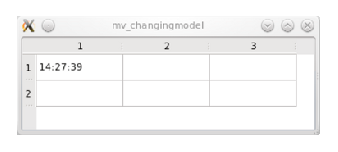
\includegraphics[width=0.5\textwidth]{clock}
\end{figure}

我们仍然使用一个只读表,但是这次内容每秒更改一次,因为我们正在显示当前时间。

(文件:examples/widgets/tutorials/modelview/3\_changingmodel/mymodel.cpp)

\begin{lstlisting}{language=C++}
QVariant MyModel::data(const QModelIndex &index, int role) const
{
    int row = index.row();
    int col = index.column();

    if (role == Qt::DisplayRole && row == 0 && col == 0)
        return QTime::currentTime().toString();

    return QVariant();
}
\end{lstlisting}

缺少一些东西来使时钟滴答作响。我们需要每秒告诉视图时间已更改,并且需要再次读取。
我们用一个计时器来做到这一点。
在构造函数中,我们将其间隔设置为1秒,然后连接其超时信号。

(文件:examples/widgets/tutorials/modelview/3\_changingmodel/mymodel.cpp)

\begin{lstlisting}{language=C++}
MyModel::MyModel(QObject *parent)
    : QAbstractTableModel(parent)
    , timer(new QTimer(this))
{
    timer->setInterval(1000);
    connect(timer, &QTimer::timeout , this, &MyModel::timerHit);
    timer->start();
}
\end{lstlisting}

(文件:examples/widgets/tutorials/modelview/3\_changingmodel/mymodel.cpp)

槽函数:

\begin{lstlisting}{language=C++}
void MyModel::timerHit()
{
    //we identify the top left cell
    QModelIndex topLeft = createIndex(0,0);
    //emit a signal to make the view reread identified data
    emit dataChanged(topLeft, topLeft, {Qt::DisplayRole});
}
\end{lstlisting}

我们通过发射 dataChanged() 信号要求视图再次读取左上角单元格中的数据。
请注意,我们没有将 dataChanged 信号显式连接到视图。这在我们调用 setModel 时自动发生。